\documentclass[11pt]{article}

\usepackage[margin=1in]{geometry}
\usepackage{amsmath,amssymb,amsthm}
\usepackage{bm}
\usepackage{algorithm}
\usepackage{algpseudocode}
\usepackage{booktabs}
\usepackage{makecell}
\usepackage{microtype}
\usepackage{graphicx}
\usepackage{tikz}
\usetikzlibrary{arrows.meta,positioning}
\usepackage[numbers,sort&compress]{natbib}
\usepackage[hidelinks]{hyperref}

\newtheorem{proposition}{Proposition}
\newtheorem{remark}{Remark}

% --- notation shortcuts ---
\newcommand{\R}{\mathbb{R}}
\newcommand{\given}{\,|\,}
\newcommand{\ind}[1]{\mathbf{1}\!\left[#1\right]}
\newcommand{\zt}{z_{\theta}}
\newcommand{\Il}{I_{\ell}}
\newcommand{\trans}{^{\top}}
\DeclareMathOperator*{\argmin}{arg\,min}
\DeclareMathOperator*{\argmax}{arg\,max}

\title{RepLeafGBM: Gradient Boosting with Raw-Feature Routing\\
and Representation-Conditioned Leaves}
\author{Masaya Kawamata}
\date{\today}

\begin{document}
\maketitle

\begin{abstract}
RepLeafGBM is a gradient-boosted tree ensemble whose trees \emph{route} on raw,
interpretable features while each \emph{leaf} predicts through a learned, frozen
representation $\zt(x)$. It occupies the space between classic gradient-boosted
decision trees (GBDTs), whose leaves emit a constant, and tabular deep learning,
which embeds features but discards the axis-aligned tree. Routing stays
axis-aligned, categorical-native, and readable; expressivity is added only inside
the leaf, as an $h$-weighted ridge fit of an affine model on $\zt(x)$. We give the
additive/Newton formulation, the constant and embedded-linear leaf models, and a
supervised \emph{pretrain-then-freeze} encoder, together with a proposition showing
that updating the encoder during boosting breaks the stage-wise additive structure
of gradient boosting---which is why the encoder is frozen. We then study the method
empirically and report an honest picture. Under a \emph{shared}
hyperparameter-optimization budget on the Grinsztajn tabular benchmarks, with significance
testing, RepLeafGBM is a competitive \emph{mid-pack} learner---not state-of-the-art on
average. Its distinctive value is in niche regimes: the representation-conditioned leaf is a
genuine, separable contribution (refitting an external GBDT's own routes with
embedded-linear leaves improves regression RMSE by $5$--$9\%$ on synthetic targets and
significantly---Wilcoxon $p=0.002$ over ten seeds, no losses---on every real regression
dataset tested), and joint vector-leaf routing with robust objectives is decisive under
target contamination (beating squared error on $10/10$ seeds at every contamination level
on all five real multi-target datasets)---where we identify and fix a scale bug in
saturated-gradient (Huber/quantile) objectives through per-output target standardization,
making them robust \emph{consistently} across target scales. Equally, we
document where the idea does \emph{not} help---binary classification (the logistic Hessian
starves the leaf-linear fit), and \emph{learned} encoders, which beat \texttt{identity} on
structured synthetic data but fail to transfer to real tabular targets. We release an
open-source implementation with parity-tested NumPy, Rust ($\sim$5.8$\times$), and
CUDA (up to 5.5$\times$) backends.
\end{abstract}

\section{Introduction}
\label{sec:intro}

Gradient-boosted decision trees (GBDTs) remain the dominant model class on tabular
data~\citep{friedman2001greedy,chen2016xgboost,ke2017lightgbm,prokhorenkova2018catboost},
and recent benchmarks confirm that they still match or outperform deep tabular models
on typical problems~\citep{grinsztajn2022why}. Their strength is the axis-aligned
split: routing on raw features handles discontinuities, interactions, missing values,
and categorical columns cheaply and interpretably. Their weakness is the
\emph{leaf}: a classic GBDT emits a constant per leaf, so a smooth within-region
effect---a price gradient, a redshift trend, a dose response---can only be
approximated by stacking many small steps.

Tabular deep learning attacks the opposite end. Numerical-feature embeddings,
notably the piecewise-linear and periodic families of \citet{gorishniy2022embeddings},
let neural models capture smooth nonlinear structure that constant-leaf trees
represent only coarsely~\citep{arik2021tabnet,popov2020node,gorishniy2021revisiting}.
But these models embed features as the \emph{input} to a deep network and discard the
axis-aligned tree, giving up the routing that makes GBDTs robust on messy tables.

RepLeafGBM is a deliberately \emph{asymmetric} hybrid that keeps both halves. Trees
route on raw features exactly as in a histogram GBDT; each leaf, instead of a
constant, holds a small ridge-regularized affine model over a learned representation
$\zt(x)$. The embedding does the smooth interpolation \emph{inside} a region, while
the representation is never used for splitting---so routing stays axis-aligned,
categorical-native, and readable, and the search never suffers an embedding-induced
dimensionality blow-up. Crucially, the encoder is fitted once before boosting and
then \emph{frozen}; we prove (Proposition~\ref{prop:freeze}) that updating it
mid-boosting would retroactively change every earlier tree's output and break the
stage-wise additive interpretation of boosting. RepLeafGBM is therefore neither a
neural network placed inside a tree nor a tree grown over embeddings.

\paragraph{Contributions.}
\begin{enumerate}
\item \textbf{The RepLeafGBM architecture} (\S\ref{sec:repleaf}--\ref{sec:leaves}):
  raw-feature routing with representation-conditioned constant and embedded-linear
  leaves, fitted in the Newton / $h$-weighted-least-squares GBDT framework, with a
  prediction-time extrapolation guard and a constant-leaf fallback.
\item \textbf{A correctness argument for freezing} (\S\ref{sec:freeze}): a proposition
  that a mid-boosting encoder update breaks stage-wise additivity, motivating the
  pretrain-then-freeze design and delimiting what alternating optimization would
  require.
\item \textbf{A supervised pretrain-then-freeze encoder} (\S\ref{sec:pretrain}) whose
  target is the negative gradient at the initial score, with an analysis of why $-g$
  (not the Newton target $-g/h$) is the right pretraining signal.
\item \textbf{Multiclass and multi-output regimes, and scale-consistent robust objectives}
  (\S\ref{sec:algorithm}, \S\ref{sec:exp-multioutput}): one-tree-per-class softmax and a
  shared-routing vector leaf that solves $K$ ridge problems from one Gram factorization,
  including robust (Huber/quantile) objectives. We identify that their saturated gradients
  under-fit large-scale targets and fix it with per-output target standardization, turning
  robust multi-output regression into a \emph{general} win under contamination.
\item \textbf{An honest empirical study} (\S\ref{sec:experiments}): a fair,
  same-HPO-budget leaderboard on the Grinsztajn tabular suites with significance testing
  (RepLeafGBM is competitive mid-pack), niche studies (leaf-channel isolation via router
  extraction; robust multi-output under contamination), and an ensemble-diversity probe. We
  report null results as prominently as wins.
\item \textbf{An open-source implementation} with parity-tested NumPy, Rust, and CUDA
  split/leaf backends.
\end{enumerate}

\section{Related work}
\label{sec:related}

\paragraph{Gradient-boosted decision trees.}
Gradient boosting~\citep{friedman2001greedy} and its second-order, regularized
formulations~\citep{friedman2000additive,chen2016xgboost} underlie modern histogram
GBDTs. LightGBM~\citep{ke2017lightgbm} contributes leaf-wise growth and gradient-based
categorical subset splits; CatBoost~\citep{prokhorenkova2018catboost} uses oblivious
(symmetric) trees as a strong regularizer and fast predictor. RepLeafGBM reuses this
routing machinery verbatim---histogram splits, Newton gain, leaf-wise/depthwise/
symmetric policies, categorical subset splits---and changes only the leaf.
NGBoost~\citep{duan2020ngboost} varies the complementary axis: it keeps simple leaves but
changes \emph{what} they predict (distributional parameters via natural gradients),
whereas RepLeafGBM changes what the leaf predicts \emph{on}; the two are compatible in
principle, though v0 does not combine them.

\paragraph{Model trees and piecewise-linear leaves.}
Replacing the constant leaf with a local linear model is a long line of work: model
trees~\citep{quinlan1992m5,wang1997m5prime}, logistic model
trees~\citep{landwehr2005lmt}, and, within boosting, gradient boosting with
piecewise-linear regression trees~\citep{shi2019gbdtpl} (implemented as LightGBM's
\texttt{linear\_tree} option). Boosted generalized additive models---intelligible
models and GA\textsuperscript{2}M, popularized as Explainable Boosting
Machines~\citep{lou2012intelligible,lou2013accurate}---also enrich the weak learner,
but with per-feature (or feature-pair) shape functions in which routing and leaf basis
are the \emph{same} raw features. All of these fit their local model in the raw (or
selected) features. RepLeafGBM's leaf instead regresses on a \emph{learned, frozen}
representation $\zt(x)$, decoupled from the routing features, of which the raw-linear
leaf is the identity-encoder special case.

\paragraph{Tabular deep learning and numerical embeddings.}
Neural tabular models embed features and learn interactions end-to-end:
TabNet~\citep{arik2021tabnet}, NODE~\citep{popov2020node}, and
FT-Transformer~\citep{gorishniy2021revisiting}. \citet{gorishniy2022embeddings} show
that piecewise-linear (PLR) and periodic numerical embeddings are the key ingredient;
these are exactly the encoder families RepLeafGBM can consume. The difference is how
the embedding is used: as the input to a deep network there, versus a frozen
\emph{leaf basis} under an explicit tree here. A separate axis is in-context tabular
prediction: TabPFN~\citep{hollmann2025tabpfn} amortizes training into a pretrained
transformer prior and excels on small datasets, without explicit routing.
\citet{grinsztajn2022why} document that tree-based models still lead on typical tabular
data; \citet{mcelfresh2023when} show that much of the apparent NN-vs-GBDT gap dissolves
under matched tuning budgets---precisely the caution our shared-budget evaluation
protocol (\S\ref{sec:exp-openml}) adopts---and the living TabArena
benchmark~\citep{erickson2025tabarena} confirms tuned GBDTs remain strong defaults.
Together these motivate keeping the tree explicit.

\paragraph{Hybrids of trees and representations.}
Deep neural decision forests~\citep{kontschieder2015deep} and NODE~\citep{popov2020node}
make routing itself soft/differentiable over learned features; DeepGBM~\citep{ke2019deepgbm}
distills GBDT structure into a network. All of these let representations influence
\emph{routing}. RepLeafGBM deliberately does the opposite: routing is a hard,
raw-feature decision tree, and the representation acts only as the regressor basis
inside each leaf---preserving GBDT routing semantics while adding leaf expressivity.

\section{Notation and gradient boosting}
\label{sec:notation}

We are given $n$ examples $\{(x_i, y_i)\}_{i=1}^{n}$ with raw feature vectors
$x_i \in \R^{d}$ (numeric and categorical entries) and targets $y_i$. A
differentiable loss $L(y, F)$ measures the discrepancy between a target and a
real-valued raw score $F$ (for $K$-way problems, $F \in \R^{K}$). Gradient
boosting~\citep{friedman2001greedy} builds an additive model stage-wise,
\begin{equation}
F_0(x) = \argmin_{c} \sum_{i=1}^{n} L(y_i, c),
\qquad
F_t(x) = F_{t-1}(x) + \eta\, f_t(x),
\label{eq:additive}
\end{equation}
where $\eta \in (0,1]$ is the learning rate and $f_t$ is the round-$t$ weak
learner. At round $t$ we expand $L$ to second order around the current score using
the per-row gradient and Hessian
\begin{equation}
g_i = \left.\frac{\partial L(y_i, F)}{\partial F}\right|_{F = F_{t-1}(x_i)},
\qquad
h_i = \left.\frac{\partial^2 L(y_i, F)}{\partial F^2}\right|_{F = F_{t-1}(x_i)} .
\end{equation}
Dropping constants, the round-$t$ objective is the quadratic
\begin{equation}
\sum_{i} \Big[\, g_i f(x_i) + \tfrac{1}{2} h_i f(x_i)^2 \,\Big] + \Omega(f)
= \tfrac{1}{2} \sum_{i} h_i \big( f(x_i) - t_i \big)^2 + \text{const} + \Omega(f),
\qquad
t_i = -\frac{g_i}{h_i},
\label{eq:newton}
\end{equation}
where $\Omega(f)$ is an $L_2$ regularizer on the leaf parameters. Equation
\eqref{eq:newton} is the workhorse identity: \emph{every} weak learner, whatever its
leaf model, is fitted by \textbf{$h$-weighted least squares on the Newton targets}
$t_i = -g_i/h_i$. For squared error ($h_i \equiv 1$, $t_i$ the residual) this is
exact rather than approximate.

\paragraph{Sample weights.}
Per-row weights $\omega_i \ge 0$ scale each loss term, so $g_i, h_i$ are replaced by
$\omega_i g_i, \omega_i h_i$ everywhere. The Newton target $t_i = -g_i/h_i$ is
unchanged but its fitting weight becomes $\omega_i h_i$; folding the weight into
$(g,h)$ before any histogram is built leaves the split and leaf kernels untouched.

\section{RepLeafGBM: raw routing and representation-conditioned leaves}
\label{sec:repleaf}

\begin{figure}[t]
\centering
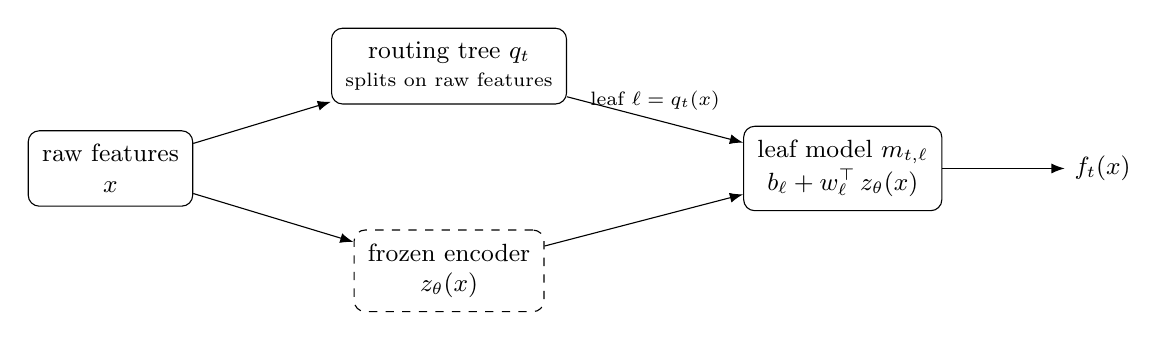
\begin{tikzpicture}[>=Latex, font=\small,
  box/.style={draw, rounded corners, align=center, inner sep=5pt},
  frozen/.style={draw, dashed, rounded corners, align=center, inner sep=5pt}]
  \node[box]    (x)    at (0,0)       {raw features\\ $x$};
  \node[box]    (tree) at (4.3,1.3)   {routing tree $q_t$\\[-1pt] {\scriptsize splits on raw features}};
  \node[frozen] (enc)  at (4.3,-1.3)  {frozen encoder\\ $\zt(x)$};
  \node[box]    (leaf) at (9.3,0)     {leaf model $m_{t,\ell}$\\[1pt] $b_\ell + w_\ell^{\top}\,\zt(x)$};
  \node         (out)  at (12.6,0)    {$f_t(x)$};
  \draw[->] (x) -- (tree);
  \draw[->] (x) -- (enc);
  \draw[->] (tree) -- node[above, font=\scriptsize] {leaf $\ell = q_t(x)$} (leaf);
  \draw[->] (enc)  -- (leaf);
  \draw[->] (leaf) -- (out);
\end{tikzpicture}
\caption{A RepLeafGBM round-$t$ weak learner. The tree $q_t$ routes $x$ to a leaf using
\emph{raw features only} (invariant I1); the \emph{frozen} encoder produces $\zt(x)$
(invariant I2); the selected leaf $\ell$ predicts the affine model $b_\ell + w_\ell^{\top}
\zt(x)$. The boosted model sums $F_T(x) = F_0 + \eta\sum_{t} f_t(x)$. The representation
never enters a split, and the encoder is fixed throughout boosting.}
\label{fig:arch}
\end{figure}

A classic GBDT weak learner is a regression tree whose leaves emit a constant.
RepLeafGBM keeps the boosting and routing machinery but upgrades the leaf. Let
$\zt : \R^{d} \to \R^{d_z}$ be an encoder producing a learned representation, fitted
once and then \emph{frozen} (Section~\ref{sec:freeze}). A round-$t$ weak learner is a
pair $(q_t, \{m_{t,\ell}\})$:
\begin{itemize}
\item a \textbf{routing tree} $q_t : \R^{d} \to \{1,\dots,L_t\}$ that maps an example
  to a leaf index using \emph{raw features only} --- the representation never enters a
  split test; and
\item a per-leaf \textbf{leaf model} $m_{t,\ell}$ evaluated on the representation
(Figure~\ref{fig:arch}), so
\begin{equation}
f_t(x) = m_{t,\,q_t(x)}\big(\zt(x)\big).
\end{equation}
\end{itemize}
With the affine (\emph{embedded-linear}) leaf of Section~\ref{sec:leaves}, the full
ensemble after $T$ rounds is
\begin{equation}
F_T(x) = F_0 + \eta \sum_{t=1}^{T}
\Big[\, b_{t,\,\ell_t(x)} + w_{t,\,\ell_t(x)}^{\!\trans}\, \zt(x) \,\Big],
\qquad \ell_t(x) = q_t(x).
\label{eq:ensemble}
\end{equation}

Two invariants define the method and are preserved throughout:
\begin{description}
\item[\textnormal{(I1) Raw-feature routing.}] Splits are chosen from raw features
  only; the tree partition is axis-aligned and human-readable, exactly as in
  LightGBM/XGBoost~\citep{ke2017lightgbm,chen2016xgboost}, and categorical columns
  route through native subset splits. The embedding dimensions are never split on.
\item[\textnormal{(I2) Frozen encoder.}] $\zt$ is fitted before boosting and held
  fixed; past leaves' parameters depend on $\zt$, so updating $\theta$ mid-boosting
  would break the stage-wise additive assumption (Section~\ref{sec:freeze}).
\end{description}
RepLeafGBM is therefore \emph{not} a neural network placed inside a tree, and
\emph{not} a tree grown over embeddings: routing remains a raw-feature decision tree,
and the learned representation acts only as the regressor basis inside each leaf.

\paragraph{Routing: split selection.}
Trees are grown greedily on histograms of the raw features, scoring a candidate split
of a node with row set $I$ into children $I_L, I_R$ by the standard Newton
gain~\citep{chen2016xgboost}
\begin{equation}
\mathrm{gain} = \frac{G_L^2}{H_L + \lambda} + \frac{G_R^2}{H_R + \lambda}
- \frac{G^2}{H + \lambda},
\qquad
G_{(\cdot)} = \!\!\sum_{i \in I_{(\cdot)}}\!\! g_i, \quad
H_{(\cdot)} = \!\!\sum_{i \in I_{(\cdot)}}\!\! h_i,
\label{eq:gain}
\end{equation}
with $\lambda = \texttt{l2\_leaf}$, \texttt{min\_samples\_leaf} enforced on both
children, and missing values routed to the left child. The growth policy
(\texttt{leafwise}~\citep{ke2017lightgbm} best-gain-first by default; also
\texttt{depthwise} and oblivious \texttt{symmetric}~\citep{prokhorenkova2018catboost})
only changes \emph{which} node is expanded next, not the per-split score; (I1) holds
for all policies.

\section{Leaf models}
\label{sec:leaves}

Given a fixed partition, each leaf is fitted independently by the $h$-weighted least
squares of \eqref{eq:newton} restricted to its rows $\Il$.

\paragraph{Constant leaf.}
The minimizer of $\sum_{i \in \Il} h_i (b - t_i)^2 + \lambda b^2$ is the
XGBoost-style damped Newton step
\begin{equation}
b_{\ell} = -\frac{\sum_{i \in \Il} g_i}{\sum_{i \in \Il} h_i + \lambda}.
\label{eq:constleaf}
\end{equation}

\paragraph{Embedded-linear leaf.}
Let $z_i = \zt(x_i)$. The leaf fits an affine model on the representation by ridge
regression~\citep{hoerl1970ridge} with an \emph{unpenalized} intercept,
\begin{equation}
\min_{b,\, w} \ \sum_{i \in \Il} h_i \big( b + w^{\!\trans} z_i - t_i \big)^2
\;+\; \lambda \lVert w \rVert^2 .
\label{eq:linleaf}
\end{equation}
Centering $z$ and $t$ by their $h$-weighted means $\bar z, \bar t$ over $\Il$
decouples the intercept and yields the ridge normal equations
\begin{equation}
\big( Z_c^{\!\trans} H Z_c + \lambda I \big)\, w = Z_c^{\!\trans} H\, t_c,
\qquad
b = \bar t - w^{\!\trans} \bar z,
\label{eq:normaleq}
\end{equation}
where $Z_c, t_c$ are the centered design and targets and $H = \mathrm{diag}(h_i)$.
Equation \eqref{eq:constleaf} is the special case $w = 0$. The \emph{raw-linear}
variant replaces $z_i$ with standardized raw numeric features.

\paragraph{Extrapolation guard.}
Each linear leaf stores the per-dimension range $[z_{\min}, z_{\max}]$ of the
embeddings it was fitted on, and predicts with $\mathrm{clip}(z, z_{\min}, z_{\max})$:
the leaf's response is its fitted affine function inside the training support and
constant outside it. Training rows lie inside by construction, so the training
trajectory is unchanged; only out-of-support queries are clamped.

\paragraph{Conditioning and fallback.}
The system \eqref{eq:normaleq} can be ill-conditioned for small or locally degenerate
leaves. The leaf falls back to the constant model \eqref{eq:constleaf} when
$\lvert \Il \rvert < \max(2\,\texttt{min\_samples\_leaf},\, d_z + 2)$, or when the
solve fails or returns non-finite weights; $\lambda > 0$ is required in practice.

\section{The frozen-encoder design and why it is necessary}
\label{sec:freeze}

Invariant (I2) is not a convenience --- it is required for the boosting objective to
remain well defined. Consider the ensemble \eqref{eq:ensemble}. Each leaf weight
$w_{t,\ell}$ was fitted against the value of $\zt$ \emph{as it stood at round $t$}.

\begin{proposition}[Encoder updates break stage-wise additivity]
\label{prop:freeze}
Suppose the encoder parameters are changed from $\theta$ to $\theta'$ at some round
$T' > t$, after trees $1,\dots,t$ have been fitted. Then
\begin{enumerate}
\item the outputs of all earlier trees $1,\dots,T'$ change retroactively, since each
  emits $b_{\cdot,\ell} + w_{\cdot,\ell}^{\!\trans} z_{\theta'}(x) \neq
  b_{\cdot,\ell} + w_{\cdot,\ell}^{\!\trans} z_{\theta}(x)$;
\item consequently the cached raw scores $F$ used to form $(g,h)$ no longer equal the
  model's actual output, so every subsequent gradient is evaluated at the wrong point;
  and
\item the interpretation of boosting as coordinate descent in function space --- each
  stage greedily fitting the current residual --- no longer holds.
\end{enumerate}
\end{proposition}

Restoring correctness after an encoder update would require re-evaluating (or
re-fitting) all earlier leaf weights and invalidating the prediction cache, i.e.\
alternating optimization between $\theta$ and the ensemble. RepLeafGBM v0 instead
adopts the simplest sound choice: \emph{fit $\zt$ once before boosting, then freeze
it}. The representation is thus a fixed, supervised feature map, and the leaf solves
\eqref{eq:normaleq} are ordinary ridge regressions against a constant basis.

\begin{remark}
Freezing also keeps the leaf fit convex and closed-form, makes training embarrassingly
reusable across rounds (the embedding $Z = \zt(X)$ is computed once), and preserves a
clean separation of concerns: the encoder owns the representation, the booster owns
gradients, tree growth, and leaf fitting.
\end{remark}

\section{Supervised encoder pretraining}
\label{sec:pretrain}

A \emph{learned} encoder is fitted once, before boosting, on a supervised target and
then frozen. The target is the \textbf{negative gradient of the loss at the constant
initial score $F_0$} --- precisely the residual the first tree would chase:
\begin{equation}
\begin{aligned}
\text{regression:} \quad & t = -g = y - \overline{y}, && h = 1,\\
\text{binary:} \quad & t = -g = y - \sigma(F_0), \\
\text{multiclass:} \quad & T = -g = \mathrm{onehot}(y) - \mathrm{softmax}(F_0) \in \R^{n\times K}, && F_{0,k} = \log \mathrm{prior}_k,\\
\text{multi-output:} \quad & T = -g = Y - \overline{Y} \in \R^{n\times K}, && F_{0,k} = \overline{Y}_{\cdot k}.
\end{aligned}
\end{equation}
A scalar target trains a $\mathrm{Linear}(d_z, 1)$ head on $\zt(x)$; an $(n,K)$ matrix
target trains a $\mathrm{Linear}(d_z, K)$ head, with the mean-squared error averaged
over rows and outputs so the representation is pushed to be linearly predictive of
every output residual at once. Each output column is standardized to unit variance so
no class/output dominates, and the head is discarded after fitting. Two choices are
worth recording.

\paragraph{Why $-g$ rather than the Newton target $-g/h$.}
Pretraining should align the representation with the loss's steepest-descent
direction; the Hessian reweighting belongs to the leaf solve, not to feature learning.
Moreover, at $F_0$ the multiclass Hessian $h_k = p_k(1-p_k)$ is \emph{column-constant}
(because $\mathrm{softmax}(F_0)$ is the row-independent prior), so $-g/h$ equals $-g$
up to a per-column scale and \textbf{coincides with it after per-output
standardization}. The two formulations are identical here, and $-g$ keeps scalar and
vector targets consistent.

\paragraph{What the encoder learns.}
At $F_0$ the multiclass target reduces to $T = \mathrm{onehot}(y) - \mathrm{prior}$, a
centered class-membership indicator. Pretraining therefore teaches $\zt$ a
representation from which class membership is \emph{linearly} recoverable --- exactly
the signal the per-class linear leaves consume.

\paragraph{Encoder families.}
The leaf basis $\zt$ is pluggable, and only its output is consumed downstream; the
booster is agnostic to how $\zt$ is produced. We use two groups. \emph{Fixed} encoders
require no learning: \texttt{identity} standardizes the raw numeric features
($z_j = (x_j - \mu_j)/\sigma_j$) and is the default; \texttt{plr} appends a fixed
per-feature piecewise-linear basis over quantile bins; \texttt{periodic} appends
random sinusoidal features; and \texttt{cross} appends a few residual-correlated
pairwise products. \emph{Learned} encoders (optional, fitted by the pretraining of
this section and then frozen) follow the numerical-embedding families of
\citet{gorishniy2022embeddings}: \texttt{torch\_plr} learns a per-feature
linear--ReLU projection over the piecewise-linear basis, \texttt{torch\_periodic}
learns the periodic frequencies, and \texttt{torch\_mlp} adds a small MLP with a raw
pass-through for cross-feature structure. Learned encoders import a deep-learning
framework only at fit time; transform and serialization are pure NumPy, so a saved
model predicts without it. If an encoder's output dimension exceeds a cap
\texttt{max\_leaf\_emb\_dim}, a fixed Gaussian random projection reduces it, bounding
the per-leaf ridge cost; \S\ref{sec:experiments} measures the practical consequences
of these choices.

\section{Algorithm}
\label{sec:algorithm}

Algorithm~\ref{alg:train} states training; Algorithm~\ref{alg:predict} states
prediction. The encoder pretraining (Section~\ref{sec:pretrain}) happens once,
before the boosting loop, and $Z = \zt(X)$ is precomputed because $\zt$ never changes.

\begin{algorithm}[t]
\caption{RepLeafGBM training}
\label{alg:train}
\begin{algorithmic}[1]
\Require data $(X, y)$; loss $L$; rounds $T$; rate $\eta$; leaf capacity / policy;
ridge $\lambda$; encoder family; optional sample weights $\omega$
\State $F_0 \gets \argmin_c \sum_i L(y_i, c)$
  \Comment{(weighted) optimal constant: mean / log-odds / class-prior / quantile}
\State $T_{\mathrm{pre}} \gets -\,\nabla_F L(y, F_0)$
  \Comment{pretraining target: residual at $F_0$ (Section~\ref{sec:pretrain})}
\State fit encoder $\theta$ on $X \!\to\! T_{\mathrm{pre}}$; \textbf{freeze} $\theta$
\State $Z \gets \zt(X)$ \Comment{precompute frozen embeddings}
\State $F \gets F_0$ \textbf{for all rows}
\For{$t = 1$ \textbf{to} $T$}
  \State $g_i \gets \partial_F L(y_i, F_i)$,\quad $h_i \gets \partial_F^2 L(y_i, F_i)$
    \Comment{scale by $\omega_i$ if weighted}
  \State $t_i \gets -\,g_i / h_i$ \Comment{Newton targets}
  \State $q_t \gets \textsc{GrowTree}(X_{\text{raw}}, g, h, \texttt{leaves}, \texttt{policy})$
    \Comment{splits on raw features via gain \eqref{eq:gain}}
  \For{each leaf $\ell$ with rows $\Il$}
    \State fit $m_{t,\ell}$ on $\big(Z_{\Il},\, t_{\Il}\big)$ with weights $h_{\Il}$
      \Comment{constant \eqref{eq:constleaf} or ridge-on-$z$ \eqref{eq:normaleq};
      fallback if ill-conditioned}
  \EndFor
  \State $f_t \gets (q_t, \{m_{t,\ell}\})$;\quad $F \gets F + \eta\, f_t(X)$
  \State \textbf{optional:} early-stop on a validation metric
\EndFor
\State \Return $\big\{F_0,\, \eta,\, (q_t, \{m_{t,\ell}\})_{t=1}^{T},\, \theta\big\}$
\end{algorithmic}
\end{algorithm}

\begin{algorithm}[t]
\caption{RepLeafGBM prediction for a query $x$}
\label{alg:predict}
\begin{algorithmic}[1]
\State $z \gets \zt(x)$;\quad $F \gets F_0$
\For{$t = 1$ \textbf{to} $T$}
  \State $\ell \gets q_t(x)$ \Comment{route on raw features (missing $\to$ left)}
  \State $F \gets F + \eta\big(b_{t,\ell} + w_{t,\ell}^{\!\trans}\,
    \mathrm{clip}(z, z_{\min}^{t,\ell}, z_{\max}^{t,\ell})\big)$
    \Comment{$w_{t,\ell} = 0$ for a constant leaf}
\EndFor
\State \Return $\phi(F)$ \Comment{output transform $\phi$: identity / $\sigma$ / softmax / $\exp$}
\end{algorithmic}
\end{algorithm}

\paragraph{Multi-class and multi-output.}
Two regimes reuse the scalar machinery above. \emph{Multiclass} (softmax) grows
\emph{one tree per class} per round on column $k$ of $(g,h)$, with
$g_k = p_k - \ind{y=k}$ and $h_k = p_k(1-p_k)$; each class tree is a scalar
RepLeafGBM learner. \emph{Multi-output} regression instead grows \emph{one shared
tree per round} that routes all $K$ outputs jointly: the split gain sums the
per-output gains \eqref{eq:gain} over a shared partition, and a linear vector leaf
solves $K$ ridge problems \eqref{eq:normaleq} that --- because the constant-Hessian
losses give $h \equiv 1$ --- share a single centered Gram factorization
$Z_c^{\!\trans} Z_c + \lambda I$ with $K$ right-hand sides.

\section{Experiments}
\label{sec:experiments}

We evaluate RepLeafGBM against the strong GBDT baselines LightGBM~\citep{ke2017lightgbm},
XGBoost~\citep{chen2016xgboost}, CatBoost~\citep{prokhorenkova2018catboost}, and
scikit-learn's histogram gradient boosting~\citep{pedregosa2011scikit}, all trained on
the same ordinal-encoded feature matrix, with multiple seeds, a fixed train/validation/
test split, and early stopping on the validation split. Lower is better throughout
(RMSE for regression, log-loss for classification, mean per-output RMSE for
multi-output). The protocol asks three questions: \textbf{(Q1)} is the
representation-conditioned leaf a real contribution, separable from routing?
\textbf{(Q2)} how does RepLeafGBM compare to tuned GBDTs on real tabular data?
\textbf{(Q3)} when do \emph{learned} encoders help? All numbers below are produced by the
benchmark and experiment harness shipped with the implementation (datasets are anchored
by OpenML~\citep{vanschoren2014openml} \texttt{data\_id}; full per-dataset tables and the
reproducibility manifest are in Appendix~\ref{app:repro}).

\subsection{The leaf-model channel, isolated (Q1)}
\label{sec:exp-routerx}

The cleanest test of the leaf idea holds \emph{routing fixed} and varies only the leaf.
We take a LightGBM model, extract its early-stopped tree routes, and refit the leaves two
ways: with LightGBM's own constant leaves, and with RepLeafGBM embedded-linear leaves
over $\zt(x)$ (router extraction; the leaves are refit by sequential replay so the
boosting consistency is preserved). Table~\ref{tab:routerx} shows that on the same routes
(ten seeds), swapping constant for embedded-linear leaves improves regression by $5.1\%$
RMSE with the identity encoder and by $9.2\%$ with a PLR encoder, while a fully native
RepLeafGBM (grown with embedded leaves interleaved) does better still with far fewer
trees. On binary data the leaf swap is neutral---a recurring theme below.

\begin{table}[t]
\centering
\caption{Leaf-model channel isolated by router extraction (mean over ten seeds; RMSE for
regression, log-loss for binary; lower is better). Holding LightGBM's routes fixed,
embedded-linear leaves improve regression---and a PLR leaf basis helps further on the
synthetic targets whose smooth per-feature structure it can represent---while the native
RepLeafGBM is best. ``n.s.'' denotes a difference within one standard deviation.}
\label{tab:routerx}
\begin{tabular}{lcccc}
\toprule
Dataset (metric) & LightGBM & \makecell{routes\\+ emb.\ leaf (id.)} & \makecell{routes\\+ emb.\ leaf (PLR)} & \makecell{RepLeafGBM\\(native)} \\
\midrule
\texttt{piecewise\_linear} (RMSE) & 0.4747 & 0.4507 \,($-5.1\%$) & 0.4309 \,($-9.2\%$) & \textbf{0.4136} \\
\texttt{friedman1} (RMSE)         & 1.1933 & 1.1690 \,($-2.0\%$) & 1.1854 \,($-0.7\%$) & \textbf{1.1216} \\
\texttt{binary\_piecewise} (log-loss) & 0.2803 & 0.2825 \,(n.s.) & 0.2833 \,(n.s.) & \textbf{0.2800} \\
\bottomrule
\end{tabular}
\end{table}

On real regression data the same isolation holds and is now formally significant:
refitting an identity-embedded linear leaf on extracted LightGBM routes improves RMSE on
\texttt{california} (median $-0.0076$, $9/1/0$ wins over ten seeds),
\texttt{diamonds} ($-0.0021$, $7/3/0$), and \texttt{wine\_quality} ($-0.0060$, $4/6/0$,
no losses), each with two-sided Wilcoxon $p=0.002$. A PLR encoder is weaker than
identity on every real dataset (significant only on \texttt{california}, and by a smaller
margin)---on real targets the gain is the linear leaf itself, not a richer
representation, reinforcing \texttt{identity} as the default (\S\ref{sec:exp-encoders});
the PLR column of Table~\ref{tab:routerx} shows the richer basis paying off only where
the target has planted smooth per-feature structure.

\subsection{Leaf models and the extrapolation guard on real data}
\label{sec:exp-guard}

On real regression data, an unguarded embedded-linear leaf can extrapolate
catastrophically when a query lands outside a leaf's training support: on
\texttt{diamonds}, a handful of $z$-outliers blew the test RMSE up to $0.276$. The
prediction-time extrapolation guard (\S\ref{sec:leaves}) clips $z$ to each leaf's fitted
range, and recovers a competitive model without changing the training trajectory
(Table~\ref{tab:guard}). With the guard---and with native categorical subset splits for
low-cardinality categoricals---embedded-linear leaves beat constant leaves on $3/3$ real
regression datasets and edge out LightGBM with native categorical handling on
\texttt{diamonds}. High-cardinality categoricals (e.g.\ \texttt{adult}, up to 41
categories) remain a place where LightGBM's categorical pipeline is ahead by $\le0.7\%$.

\begin{table}[t]
\centering
\caption{Real-data regression RMSE ($\downarrow$; log1p target for \texttt{house\_sales}/
\texttt{diamonds}, 15k rows, 2 seeds). The extrapolation guard resolves the
\texttt{diamonds} blow-up and helps everywhere; categorical subset splits then give
\texttt{diamonds} the win over LightGBM with native categoricals. \texttt{california} has
no categorical features.}
\label{tab:guard}
\begin{tabular}{lcccc}
\toprule
Dataset & \makecell{embedded leaf\\(pre-guard)} & \makecell{+ extrapolation\\guard} & \makecell{+ categorical\\subset splits} & \makecell{LightGBM\\(native cat.)} \\
\midrule
\texttt{california}  & 0.4743 & 0.4594 & --- & 0.4628 \\
\texttt{house\_sales}& 0.1681 & 0.1667 & 0.1660 & \textbf{0.1652} \\
\texttt{diamonds}    & 0.2760 & 0.0953 & \textbf{0.0940} & 0.0948 \\
\bottomrule
\end{tabular}
\end{table}

\subsection{Real-data leaderboard under a shared HPO budget (Q2)}
\label{sec:exp-openml}

A credible comparison must tune \emph{every} model under the same budget on a recognized
suite. We evaluate on the four Grinsztajn et al.~\citep{grinsztajn2022why} tabular
benchmarks---numerical and categorical $\times$ regression and classification (OpenML
study identifiers 336/337/335/334; $19/16/17/7$ datasets)---under a uniform protocol: each
model family (RepLeafGBM, LightGBM, XGBoost, CatBoost, scikit-learn HistGB) is tuned by
Optuna TPE~\citep{akiba2019optuna} with an \emph{identical} number of trials ($50$ trials
$\times$ $5$ seeds), a $70/15/15$ split, and a 10k-row training cap; there is no
tuned-versus-default asymmetry. We report mean ranks with Friedman tests, Nemenyi
critical-difference diagrams, Wilcoxon signed-rank tests, and bootstrap confidence
intervals~\citep{demsar2006statistical}; a result is highlighted only when it is both
statistically significant ($p<\alpha$) and exceeds a minimum-relevant-difference band.
To keep the comparison symmetric, \emph{all} models---including RepLeafGBM---are fit on the
same ordinal-encoded matrix, so RepLeafGBM's native categorical subset splits are disabled
here: categorical performance is therefore fair, but native-categorical handling is left
untested.

The honest summary (Table~\ref{tab:openml}) is that RepLeafGBM is a \emph{consistent
mid-pack} learner. Its mean rank is $3.18$--$3.43$ out of five in \emph{every} suite; it is
never the leader, and it is never both significantly \emph{and} practically worse than the
best baseline, nor significantly better (on numerical regression the Wilcoxon test against
the best baseline is $p=0.055$, not significant). The categorical suites are statistically
flat (Friedman $p=0.375$ and $0.788$; the categorical-classification suite has only seven
datasets and correspondingly low power). RepLeafGBM is thus competitive but not
state-of-the-art on average---a useful, honestly-positioned tabular learner whose
distinctive value lies in the niche regimes studied below, not in the aggregate
leaderboard. Full per-dataset tables and the critical-difference diagrams
(Figure~\ref{fig:cd}) are produced by the shipped leaderboard harness
(Appendix~\ref{app:repro}).

\begin{figure}[t]
\centering
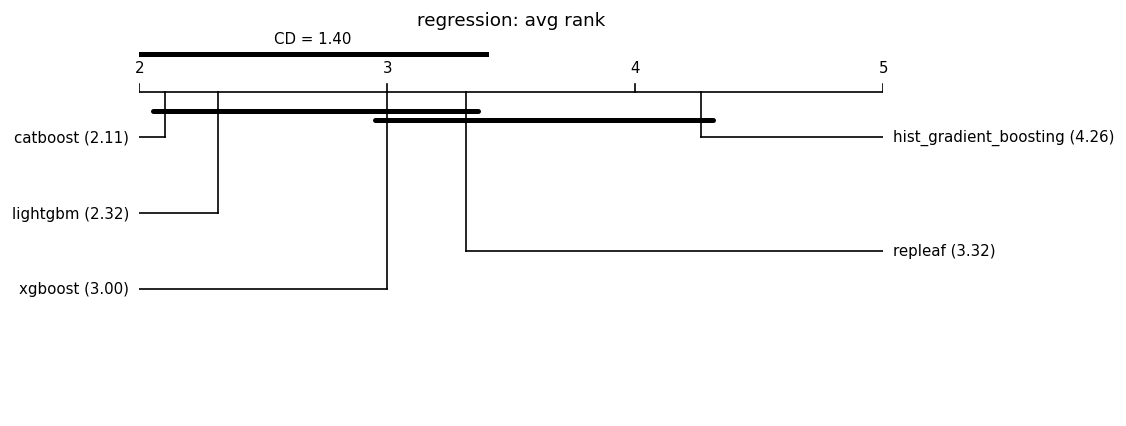
\includegraphics[width=0.49\linewidth]{figures/leaderboard-cd-grinsztajn_num_reg.png}\hfill
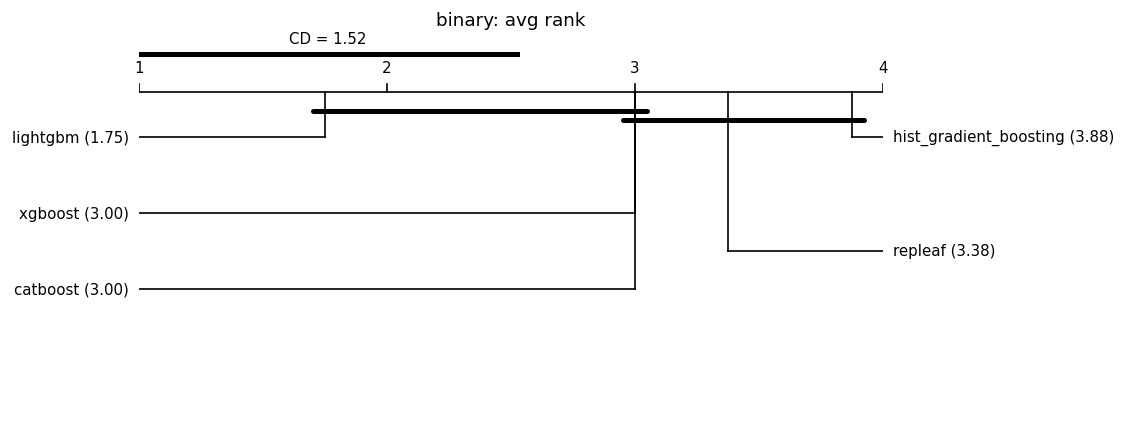
\includegraphics[width=0.49\linewidth]{figures/leaderboard-cd-grinsztajn_num_cls.png}\\[2pt]
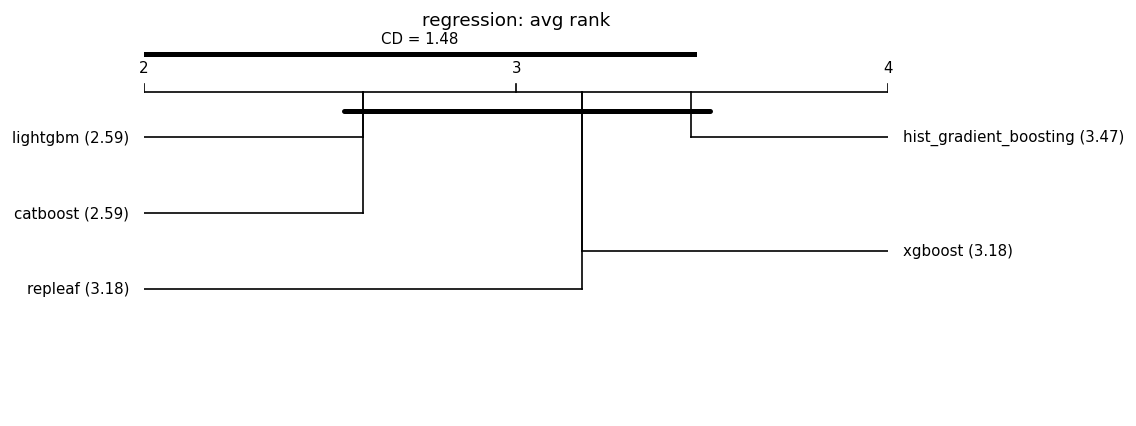
\includegraphics[width=0.49\linewidth]{figures/leaderboard-cd-grinsztajn_cat_reg.png}\hfill
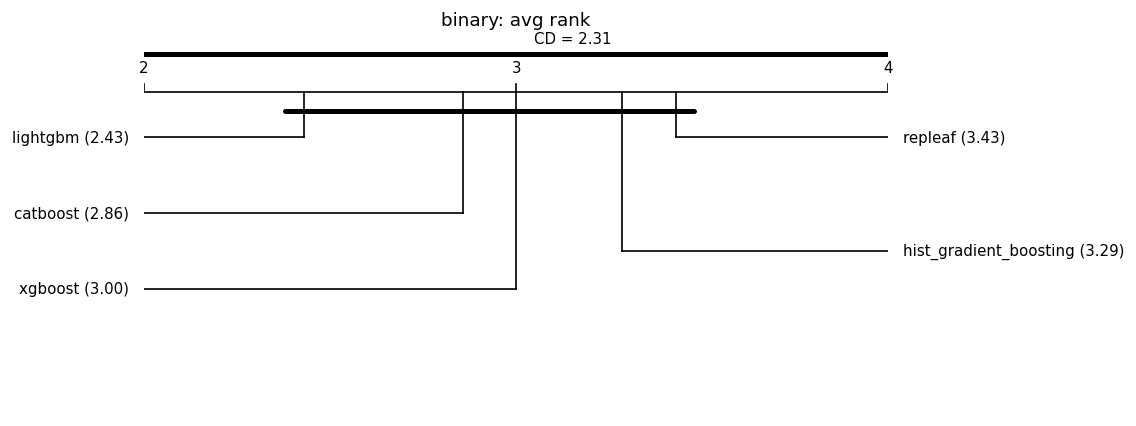
\includegraphics[width=0.49\linewidth]{figures/leaderboard-cd-grinsztajn_cat_cls.png}
\caption{Critical-difference diagrams (Nemenyi, $\alpha{=}0.05$) for the four Grinsztajn
suites under the shared HPO budget. Models joined by a bar are not statistically
separable. RepLeafGBM sits mid-pack in every suite and is never separated from the leading
GBDTs; the categorical suites are statistically flat.}
\label{fig:cd}
\end{figure}

\begin{table}[t]
\centering
\caption{Grinsztajn suites under a shared HPO budget: RepLeafGBM mean rank ($\downarrow$;
among five tuned model families, $5$ seeds). RepLeafGBM is mid-pack in every suite, with no
significant-and-practical win or loss against the best baseline; the categorical suites are
statistically flat. The Friedman $p$ is over all five models.}
\label{tab:openml}
\begin{tabular}{lcc}
\toprule
Grinsztajn suite (\# datasets) & RepLeafGBM mean rank (of $5$) & Friedman $p$ \\
\midrule
Numerical regression (19)      & $3.32$ & $1.6\times10^{-4}$ \\
Numerical classification (16)  & $3.38$ & $3.3\times10^{-3}$ \\
Categorical regression (17)    & $3.18$ & $0.375$ (flat) \\
Categorical classification (7) & $3.43$ & $0.788$ (flat) \\
\bottomrule
\end{tabular}
\end{table}

\subsection{Encoders: synthetic structure vs.\ real transfer (Q3)}
\label{sec:exp-encoders}

Learned encoders behave as \emph{specialists}, not as a better default
(Table~\ref{tab:encoders}). On synthetic targets with planted smooth/oscillatory
per-feature structure (\texttt{periodic\_mix}), the learned \texttt{torch\_periodic}
encoder beats \texttt{identity} by $13\%$; on a target dominated by a feature product
(\texttt{interaction\_mix}, not shown), interaction-aware encoders (\texttt{cross},
$0.460$; \texttt{torch\_mlp}, $0.537$) beat \texttt{identity} ($0.615$). But on every real
dataset---and on \texttt{friedman1}, whose $\sin(\pi x_1 x_2)$ interaction no per-feature
encoder can represent---\texttt{identity} is best. Adding validation-based early stopping
and weight decay to the pretraining loop does not change this picture. The reading is that
the raw-feature router already captures whatever structure these encoders extract from
real targets, so the extra capacity only adds variance; \texttt{identity} is the right
default and learned encoders are tools for targets with \emph{known} structure that trees
route poorly.

\begin{table}[t]
\centering
\caption{Encoder comparison with embedded-linear leaves (RMSE, $\downarrow$). Learned
encoders win on structured synthetic data but do not transfer to real tabular targets;
\texttt{identity} (the default) is best on all real datasets and on the interaction-heavy
\texttt{friedman1}.}
\label{tab:encoders}
\begin{tabular}{lccc}
\toprule
Dataset & \texttt{identity} & \texttt{torch\_periodic} & \texttt{torch\_plr} \\
\midrule
\texttt{periodic\_mix} (synthetic) & 0.3933 & \textbf{0.3405} & 0.3871 \\
\texttt{friedman1} (synthetic)     & \textbf{1.1282} & 1.2395 & 1.1655 \\
\texttt{california} (real)         & \textbf{0.4594} & 0.4748 & 0.4628 \\
\texttt{house\_sales} (real)       & \textbf{0.1660} & 0.1758 & 0.1682 \\
\texttt{diamonds} (real)           & \textbf{0.0940} & 0.0986 & 0.0953 \\
\bottomrule
\end{tabular}
\end{table}

\subsection{Multi-output regression and robust objectives}
\label{sec:exp-multioutput}

A single shared routing tree with vector leaves lets all outputs share one Gram
factorization (\S\ref{sec:algorithm}). On clean data (Table~\ref{tab:multioutput}) it is
decisively best on synthetic multi-output targets and beats LightGBM/HistGB on the real
energy-efficiency task, though tuned per-output CatBoost/XGBoost still lead there.

\paragraph{Robust objectives under contamination.} The constant-Hessian robust objectives
are RepLeafGBM's clearest empirical edge. We inject heavy-tailed outliers (at $8\sigma$)
into a fraction $\{0,4,8,16\%\}$ of the training targets and score on clean test data,
across five real multi-target datasets---energy-efficiency, jura, water-quality, rf1, and
scm20d---and a synthetic control, with squared, Huber~\citep{huber1964robust}, and median
(quantile, $\tau{=}0.5$) objectives over ten seeds. The result is uniform: on \emph{every}
dataset and at \emph{every} nonzero contamination level, both Huber and quantile beat
squared error on all ten seeds (two-sided Wilcoxon $p=0.002$, $10/0/0$), with effect sizes
of multiples of the target standard deviation---e.g.\ on energy at $8\%$ contamination the
median objective attains $2.40$ RMSE (Huber $3.70$) versus $12.92$ for squared error, a
$3.5$--$5.4\times$ reduction.

\paragraph{A scale-consistency fix for saturated-gradient objectives.} The two large
multi-target sets (rf1, scm20d) initially \emph{contradicted} this picture: Huber and
quantile \emph{lost} to squared error at low contamination ($4$--$8\%$), winning only at
$16\%$. The cause is a scale bug, not a robustness failure. Huber's gradient is clipped to
$\pm\delta$ and quantile's is $\pm\tau$, so the per-tree update is bounded; with a fixed
$\delta=1$ the effective ratio $\delta/\sigma$ varies by ${\sim}25\times$ across these
datasets (energy ${\approx}0.1$, scm20d ${\approx}0.004$). On large-scale targets (scm20d
per-output $\sigma{\approx}250$, rf1 ${\approx}60$) the bounded update cannot traverse the
target range within $n_\text{estimators}$ trees, so the model severely under-fits even on
\emph{clean} data---on rf1 the clean Huber RMSE is $21.1$ versus $1.5$ for squared error
(${\sim}15\times$). The fix makes the objective scale-consistent: we standardize the target
per output by its median and $1.4826\cdot\mathrm{MAD}$ before boosting, fit in the
standardized space, and un-standardize predictions, so $\delta=1$ corresponds to one
robust-$\sigma$ on every target. This removes the clean-fit penalty (rf1
$15.0\times{\rightarrow}0.9\times$, scm20d $2.4\times{\rightarrow}1.0\times$; at ten seeds
the clean Huber fit is now slightly \emph{better} than squared on both) and restores
robustness on rf1 and scm20d under contamination (rf1 at $16\%$: squared $27.8$ vs.\
standardized quantile $3.0$; scm20d at $16\%$: squared $286$ vs.\ standardized Huber
$136$), turning robust multi-output regression from a dataset-dependent into a
\emph{general} win---the uniform $10/0/0$, $p=0.002$ sweep above is measured \emph{with}
this fix in place. The standardization is applied automatically for the Huber and quantile
objectives. The one honest trade-off is on small-scale targets (energy, $\sigma{\approx}10$),
where the un-standardized objective's accidentally-aggressive clipping had been \emph{more}
robust at heavy contamination; standardization gives up a little peak robustness there
(Huber at $16\%$: $5.6$ versus squared error's $19.2$; the median objective reaches $3.1$),
and a sub-unit $\delta/\sigma$ ratio could recover it.

\begin{table}[t]
\centering
\caption{Multi-output regression, clean leaderboard: mean per-output RMSE ($\downarrow$,
5 seeds). RepLeafGBM uses one shared routing tree with vector leaves; the baselines fit one
model per output.}
\label{tab:multioutput}
\begin{tabular}{lcccc}
\toprule
Setting & RepLeafGBM & CatBoost & XGBoost & LightGBM \\
\midrule
\texttt{energy} (real, clean)     & 1.319 & \textbf{0.802} & 0.891 & 1.709 \\
synthetic ($K{=}3$, clean)        & \textbf{0.585} & 0.611 & 0.943 & 0.822 \\
\bottomrule
\end{tabular}
\end{table}

\subsection{Systems: backends}
\label{sec:exp-systems}

The split search and leaf fit run behind a backend interface with three
implementations. The optional Rust backend gives $\sim$5.8$\times$ faster constant-leaf
training than the NumPy reference while staying \emph{bitwise} parity-tested. An optional
CUDA backend (CuPy) accelerates wide and multi-output histograms; on an NVIDIA T4 it ranges
from no gain on narrow problems (launch-bound) to $5.5\times$ on wide multi-output
(Table~\ref{tab:gpu}), and is parity-tested at \texttt{allclose} (GPU atomic-add reordering
precludes bitwise equality).

\begin{table}[t]
\centering
\caption{CUDA vs.\ NumPy fit time (seconds, 30 trees, NVIDIA T4). Speedup $=$
NumPy/CUDA. GPU pays off on wide and multi-output histograms; narrow problems are
launch-bound.}
\label{tab:gpu}
\begin{tabular}{lccc}
\toprule
Task (features) & NumPy & CUDA & speedup \\
\midrule
binary (30)            & 2.34  & 2.44  & 0.96$\times$ \\
binary (200)           & 11.18 & 6.36  & 1.76$\times$ \\
regression (200)       & 11.51 & 7.03  & 1.64$\times$ \\
multiclass, $C{=}5$ (200) & 43.70 & 21.67 & 2.02$\times$ \\
multi-output, $K{=}5$ (200) & 52.79 & 9.59 & \textbf{5.50$\times$} \\
\bottomrule
\end{tabular}
\end{table}

\subsection{Further ablations}
\label{sec:exp-ablations}

Three results are reported as null/negative, which we consider part of an honest account.
\textbf{Growth policy:} oblivious (\texttt{symmetric}) trees win $10/12$ synthetic cells,
but the synthetic generators plant exactly the low-order globally-shared thresholds that
oblivious trees represent best, and we have no real-data evidence; the default therefore
stays \texttt{leafwise}. \textbf{Adaptive leaf selection:} a per-leaf leave-one-out gate
between constant and embedded-linear leaves~\citep{golub1979gcv} tracks the better of the
two but never separates from it by more than one standard deviation---a robust opt-in
hedge, not a general improvement (it is nonetheless the best-ranked RepLeafGBM arm on the
OpenML classification suite, Table~\ref{tab:openml}). \textbf{Binary classification:} no
reweighting, Hessian-floor, or $\ell_2$ remedy makes embedded-linear leaves beat constant
leaves on binary tasks (consistent across $16$ configuration--dataset cells); we trace this
to the logistic Hessian $h=p(1-p)$ shrinking the leaf-linear signal, and recommend
\texttt{constant} leaves for binary problems.

\section{Discussion}
\label{sec:rationale}

\paragraph{Two complementary channels.}
RepLeafGBM separates \emph{where to be local} from \emph{how to predict locally}.
Routing (I1) supplies axis-aligned, categorical-native, interpretable locality at GBDT
cost; the leaf model supplies smooth, non-linear response \emph{within} a region via a
learned basis. A constant-leaf GBDT can only approximate a smooth effect (e.g.\ a
photometric color or a redshift trend) by many small steps; an embedded-linear leaf
captures it directly through $w^{\!\trans} z$. Because explicit engineered features
enter the leaf's linear model, arithmetic features can help even though the
\emph{splits} are scale-invariant --- a property absent from constant-leaf GBDTs.

\paragraph{Positioning.}
The routing half is the histogram GBDT of
LightGBM/XGBoost/CatBoost~\citep{ke2017lightgbm,chen2016xgboost,prokhorenkova2018catboost}.
The leaf half borrows from tabular deep learning, where piecewise-linear and periodic
numeric \emph{embeddings} improve neural tabular models~\citep{gorishniy2022embeddings};
RepLeafGBM consumes such an embedding as a frozen leaf basis rather than as the input to a
deep network, keeping the tree explicit. Oblivious (\texttt{symmetric}) trees connect it to
CatBoost-style regularized routing~\citep{prokhorenkova2018catboost}.

\paragraph{RepLeafGBM as an ensemble member.}
Because RepLeafGBM is architecturally distinct from a standard GBDT, a natural question is
whether it adds value inside an ensemble of tuned models. Averaging it into a tuned-GBDT
blend never hurts, and on numerical regression it yields a sign-consistent improvement
(Wilcoxon $p=0.0446$, winning or tying on all $19$ datasets); but the effect is practically
negligible (only one dataset clears the relevance band, and the bootstrap mean-gain interval
straddles zero), and its prediction-error decorrelation from the GBDTs is marginal
($\Delta r{\approx}0.002$) because it still routes on raw features. The robustly-supported
finding is the generic one---ensembling beats the validation-selected best single model on
most datasets---rather than a RepLeafGBM-specific diversity benefit. RepLeafGBM is thus a
distinct blend member that never degrades an ensemble, with a diversity premium that is real
in sign but small in magnitude.

\paragraph{When the leaf channel helps.}
The experiments draw a consistent line. The embedded-linear leaf earns its keep when a
region carries a \emph{smooth} effect that a constant cannot capture but a
low-dimensional affine model on $\zt(x)$ can: real regression with the extrapolation guard
(\S\ref{sec:exp-guard}), an external GBDT's own routes refit with embedded leaves
(\S\ref{sec:exp-routerx}), and---most decisively---robust multi-output regression under
target contamination (\S\ref{sec:exp-multioutput}). It does \emph{not} help binary
classification: the logistic Hessian $h=p(1-p)\to0$ in confident regions starves the
$h$-weighted ridge fit, so the leaf-linear weights chase noise and constant leaves are both
more accurate and cheaper. This dichotomy---linear leaves pay off exactly when the Newton
targets carry recoverable smooth structure---is the paper's main practical takeaway.

\paragraph{Interpretability and the frozen-encoder trade-off.}
Because routing is a raw-feature decision tree, the partition is exactly as inspectable as a
LightGBM/XGBoost model; the representation enters only the within-leaf prediction, so the
``which leaf and why'' explanation is unchanged. Freezing the encoder
(Proposition~\ref{prop:freeze}) is what keeps each leaf solve a convex, closed-form ridge
regression and the boosting loop a coordinate descent in function space. The price is that
the representation cannot co-adapt with the ensemble; lifting it would require alternating
optimization with re-evaluation of earlier leaves and prediction-cache invalidation, which
we leave to future work (\S\ref{sec:limitations}).

\section{Limitations and future work}
\label{sec:limitations}

\emph{Method.}
(i) The Newton-target leaf fit is a second-order approximation for non-squared losses; no
line search or leaf-wise damping beyond $\lambda$ is performed. (ii) The encoder is frozen:
the alternating optimization that would let $\theta$ co-adapt with the ensemble
(\S\ref{sec:freeze}) is future work. (iii) If the encoder's output dimension exceeds a cap
\texttt{max\_leaf\_emb\_dim}, a random projection is applied, which preserves structure only
in expectation and can dilute informative dimensions. (iv) Histogram bin edges are computed
once per fit (no per-node re-quantization), and native training routes missing values left
at every split rather than learning a default direction.

\emph{Evaluation.}
(v) Our baselines are GBDTs and scikit-learn; we have not yet benchmarked against neural
tabular models such as TabNet~\citep{arik2021tabnet}, NODE~\citep{popov2020node}, or
FT-Transformer~\citep{gorishniy2021revisiting}, so the positioning relative to tabular deep
learning is argued rather than measured. (vi) The fair leaderboard uses five seeds and fifty
HPO trials per model (a ten-seed replication is the obvious firming-up step); the two niche
studies (robust multi-output, router extraction) were rerun at ten seeds and are
significant (two-sided Wilcoxon $p=0.002$), but the smaller synthetic and guard studies
remain five-seed and should be read as indicative. (vii) The per-output
target standardization that makes robust objectives scale-consistent gives up a little peak
robustness on small-scale targets; a tuned sub-unit $\delta/\sigma$ ratio is left to future
work. (viii) Two empirical questions are open: why joint vector-leaf routing trails
per-output CatBoost/XGBoost on \emph{clean} real multi-output data, and whether the
oblivious-tree advantage survives on real data under a fair capacity match. (ix)
High-cardinality categorical features still trail LightGBM's native categorical pipeline, and
the leaderboard's symmetric ordinal encoding leaves RepLeafGBM's native categorical splits
untested.

\section{Conclusion}
\label{sec:conclusion}

RepLeafGBM keeps the raw-feature, axis-aligned routing that makes GBDTs strong on tabular
data and adds expressivity only inside the leaf, as an $h$-weighted ridge fit of an affine
model on a learned, frozen representation. Freezing the encoder is not a convenience but a
correctness requirement: updating it mid-boosting breaks the stage-wise additive structure
of gradient boosting (Proposition~\ref{prop:freeze}). Empirically, under a
shared HPO budget on the Grinsztajn suites RepLeafGBM is a competitive \emph{mid-pack}
learner rather than a state-of-the-art one; its distinctive value is in niche regimes---the
representation-conditioned leaf is a real, separable contribution that improves an external
GBDT's own routes, and joint vector-leaf routing with scale-consistent robust objectives is a
decisive, general win under target contamination. We report candidly where the idea does not
help, namely binary classification and the transfer of \emph{learned} encoders to real
tabular targets. We hope
the explicit separation of \emph{where to be local} (raw routing) from \emph{how to predict
locally} (a representation-conditioned leaf), together with an honest map of when each
channel pays off, is a useful point in the design space between gradient-boosted trees and
tabular deep learning.

\section*{Acknowledgments}
The RepLeafGBM library and this manuscript were developed with extensive use of AI coding and
research assistants---primarily Anthropic's Claude (Fable~5 and Opus~4.8) via Claude Code, and
OpenAI's GPT-5.5---for implementation, architectural design, running and analyzing the
experiments, and drafting the paper. In line with arXiv's policy, these tools are not authors;
all design decisions, experimental verification, and the final content are the author's
responsibility.

\appendix

\section{Objectives}
\label{app:objectives}

Each objective supplies a per-row gradient $g_i$ and Hessian $h_i$ (used in the split gain
and as the leaf-fit weights), an optimal constant initial score $F_0$, and an output
transform $\phi$ (Table~\ref{tab:objectives}). All leaves are then fitted by $h$-weighted
least squares on the Newton targets $t_i=-g_i/h_i$ (\S\ref{sec:notation}). Here
$p=\sigma(F)$ for binary, $p_k=\mathrm{softmax}(F)_k$ for multiclass, and $\mu=e^{F}$ for
Poisson; for the quantile loss $g_i=1-\alpha$ where $F\ge y$ and $-\alpha$ otherwise.
Multiclass grows one tree per class per round; multi-output grows one shared tree per round
with vector leaves (constant-Hessian losses only).

\begin{table}[h]
\centering
\small
\caption{Objective definitions implemented by RepLeafGBM.}
\label{tab:objectives}
\begin{tabular}{lcccc}
\toprule
Objective & $g_i$ & $h_i$ & $F_0$ & $\phi$ \\
\midrule
Regression (squared)  & $F-y$ & $1$ & $\overline{y}$ & identity \\
Binary (logistic)     & $p-y$ & $p(1-p)$ & $\log\frac{\bar p}{1-\bar p}$ & $\sigma$ \\
Huber                 & $\mathrm{clip}(F-y,\pm\delta)$ & $1$ & $\mathrm{median}(y)$ & identity \\
Quantile ($\alpha$)   & $(1-\alpha)\,/\,{-}\alpha$ & $1$ & $Q_{\alpha}(y)$ & identity \\
Poisson               & $\mu-y$ & $\mu$ & $\log\overline{y}$ & $\exp$ \\
Multiclass (softmax)  & $p_k-\ind{y=k}$ & $p_k(1-p_k)$ & $\log\mathrm{prior}_k$ & softmax \\
Multi-output (squared)& $F-Y$ & $1$ & $\overline{Y}_{\cdot k}$ & identity \\
\bottomrule
\end{tabular}
\end{table}

\section{Reproducibility and additional results}
\label{app:repro}

\paragraph{Leaderboard manifest (Table~\ref{tab:openml}, Figure~\ref{fig:cd}).}
The fair-budget leaderboard runs the four Grinsztajn suites, anchored by OpenML
study ids $336$ (numerical regression, $19$ datasets), $337$ (numerical
classification, $16$), $335$ (categorical regression, $17$), and $334$ (categorical
classification, $7$). Every model family---LightGBM, XGBoost, CatBoost, scikit-learn
HistGradientBoosting, and RepLeafGBM (whose search space spans
constant/embedded-linear/adaptive leaves and identity/PLR encoders)---receives the
\emph{same} budget of $50$ Optuna TPE trials per dataset, selected on a validation
split and scored once on a held-out test split ($70/15/15$, stratified for
classification), over five seeds, with datasets capped at $10{,}000$ rows. All models
are fit on the identical ordinal-encoded matrix (RepLeafGBM's native categorical subset
splits are disabled for symmetry). Significance uses Friedman tests with Nemenyi
critical-difference diagrams, per-pair Wilcoxon signed-rank tests, and bootstrap
confidence intervals; results count only when significant \emph{and} above a
minimum-relevant-difference band. The resumable ledger, per-dataset tables, and the
harness that produced every number ship with the open-source release. The
leaf-channel isolation (Table~\ref{tab:routerx}) and robust multi-output
(\S\ref{sec:exp-multioutput}) studies use ten seeds. Package versions: Python 3.11,
numpy 1.23.5, scikit-learn 1.2.0, lightgbm 4.6.0, xgboost 3.2.0, catboost 1.2.10,
torch 2.9.1. The NumPy and Rust backends are parity-tested \emph{bitwise} (identical
histograms, leaf fits, and predictions); the CUDA backend is parity-tested at
\texttt{allclose} because GPU atomic-add reordering precludes bitwise equality.

\paragraph{Legacy breadth study (superseded).}
Tables~\ref{tab:openml-full} and~\ref{tab:synthetic} are retained from an earlier,
\emph{unequal-tuning} breadth study and are \textbf{not} the evidence behind
Table~\ref{tab:openml}: they predate the shared-HPO-budget leaderboard above and use a
different protocol---seeds $\{0,1,2\}$, a $60/20/20$ split, early stopping after $25$
rounds, at most $6{,}000$ rows, and hand-chosen model configurations; datasets are
anchored by OpenML \texttt{data\_id}: \texttt{house\_sales} (42731), \texttt{diamonds}
(42225), \texttt{wine\_quality} (287), \texttt{credit\_g} (31), \texttt{phoneme} (1489),
\texttt{adult} (1590), \texttt{wine} (187), \texttt{vehicle} (54), plus the scikit-learn
\texttt{california} set; multi-output uses energy-efficiency (1472). We keep them for
breadth (per-dataset numbers across nine datasets and eleven model arms) and because the
multiclass observation below is not covered by the leaderboard suites. Tuned GBDTs lead
the regression and binary datasets, while RepLeafGBM with embedded-linear leaves wins both
multiclass datasets among the models shown (\texttt{wine} outright across all models).

\begin{table}[h]
\centering
\small
\caption{Per-dataset OpenML primary metric ($\downarrow$; RMSE for regression, log-loss for
classification; 3 seeds). RL $=$ RepLeafGBM (constant / embedded-linear / adaptive leaves,
\texttt{identity} encoder). Bold $=$ best among the models shown.}
\label{tab:openml-full}
\begin{tabular}{lcccccc}
\toprule
Dataset & CatBoost & LightGBM & XGBoost & RL-const & RL-emb & RL-adapt \\
\midrule
\multicolumn{7}{l}{\emph{Regression} (RMSE)}\\
\texttt{california}    & \textbf{0.5013} & 0.5119 & 0.5139 & 0.5110 & 0.5080 & 0.5109 \\
\texttt{house\_sales}  & \textbf{0.1654} & 0.1712 & 0.1725 & 0.1719 & 0.1775 & 0.1721 \\
\texttt{diamonds}      & 0.1064 & \textbf{0.1035} & 0.1058 & 0.1095 & 0.1114 & 0.1108 \\
\texttt{wine\_quality} & 0.6542 & \textbf{0.6479} & 0.6499 & 0.6521 & 0.6505 & 0.6514 \\
\midrule
\multicolumn{7}{l}{\emph{Binary} (log-loss)}\\
\texttt{credit\_g}     & \textbf{0.5126} & 0.5365 & 0.5304 & 0.5491 & 0.5419 & 0.5405 \\
\texttt{phoneme}       & \textbf{0.2584} & 0.2668 & 0.2756 & 0.2697 & 0.2680 & 0.2659 \\
\texttt{adult}         & 0.3154 & 0.3167 & \textbf{0.3144} & 0.3235 & 0.3281 & 0.3239 \\
\midrule
\multicolumn{7}{l}{\emph{Multiclass} (log-loss)}\\
\texttt{wine}          & 0.1258 & 0.1629 & 0.1428 & 0.1083 & \textbf{0.0947} & 0.1013 \\
\texttt{vehicle}       & 0.5025 & 0.4995 & 0.5313 & 0.5194 & \textbf{0.4985} & 0.5053 \\
\bottomrule
\end{tabular}
\end{table}

\paragraph{Synthetic leaderboard.}
Table~\ref{tab:synthetic} reports an indicative large-synthetic benchmark
($n{=}10{,}000$, 20 features; single configuration, not multi-seed-averaged), showing
RepLeafGBM is competitive with the tuned GBDTs on synthetic regression and binary tasks.

\begin{table}[h]
\centering
\caption{Indicative large-synthetic benchmark ($n{=}10$k, 20 features). Regression RMSE and
binary log-loss ($\downarrow$). Single configuration; not a multi-seed leaderboard.}
\label{tab:synthetic}
\begin{tabular}{lcc}
\toprule
Model & Regression RMSE & Binary log-loss \\
\midrule
CatBoost                      & \textbf{0.390} & \textbf{0.256} \\
HistGradientBoosting          & 0.407 & 0.258 \\
LightGBM                      & 0.413 & 0.258 \\
RepLeafGBM (constant)         & 0.405 & 0.260 \\
RepLeafGBM (embedded-linear)  & 0.400 & 0.279 \\
\bottomrule
\end{tabular}
\end{table}

\bibliographystyle{plainnat}
\bibliography{references}

\end{document}
